\chapter{Nós}

\begin{center}
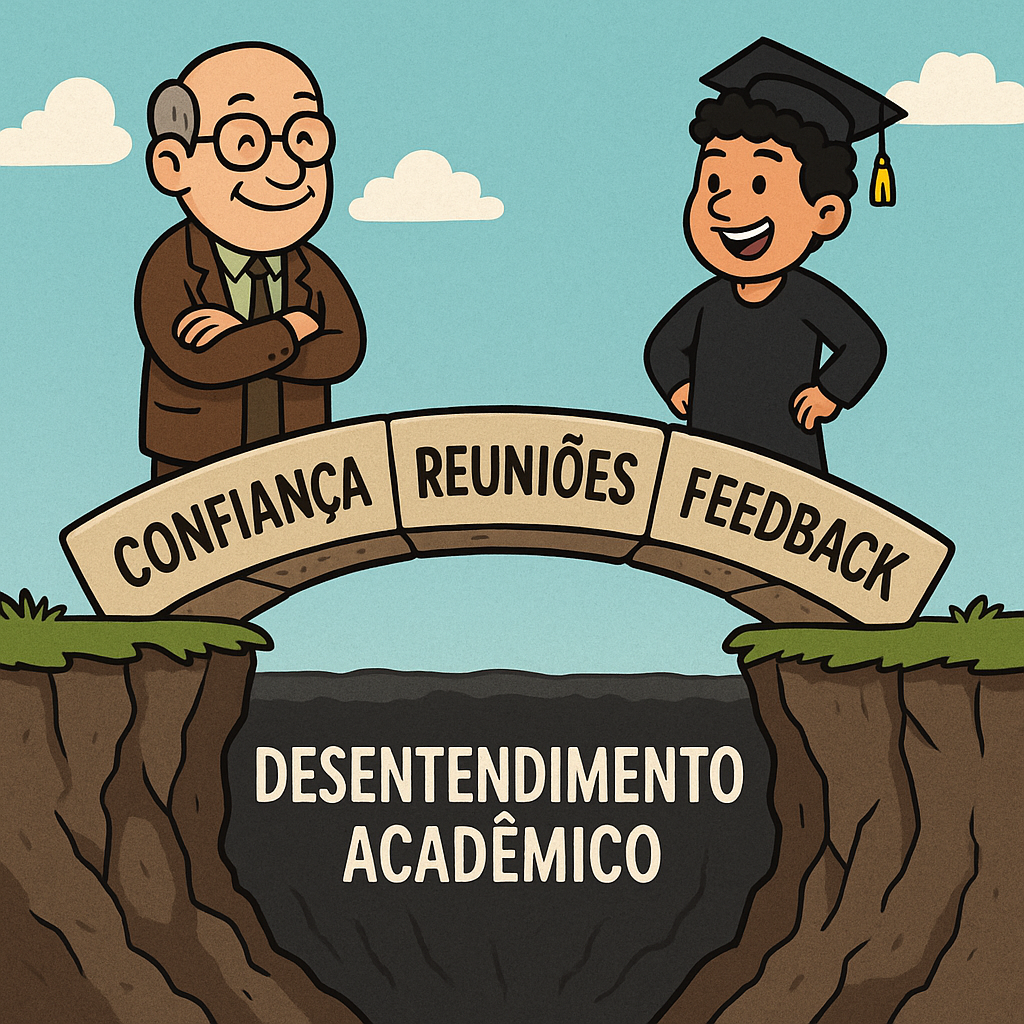
\includegraphics[width=0.5\linewidth]{Images/nos.png}    
\end{center}
\vspace{0.5cm}

\section{Eu - O Autor e Um Orientador}

Eu sou professor de graduação e pós-graduação, doutor, engenheiro e orientador em teses, dissertações e projetos finais. Tenho 30 anos de experiência nessa atividade. Para chegar a essa posição eu também tive que defender um projeto final e uma tese\footnote{Eu nunca fiz um mestrado!}. Vi também amigos meus passarem por essa experiência. Acompanho meus alunos e alunos de outros professores.

Falo com diferentes perspectivas. A primeira é de um autor genérico, descrevendo como as coisas são, ou como deviam ser. A segunda é como orientador, descrevendo como eu quero que as coisas sejam. A terceira é como professor do Programa de Engenharia de Sistemas da Coppe/UFRJ, trazendo informações específicas dessa instituição.

A maior parte do texto é atemporal. Muito pouco mudou nas relações humanas nos últimos 40 anos em que estou na academia, desde minha graduação. A tecnologia mudou a forma, mas a essência é a mesma. A parte relacionada a regras específicas sempre sofre com o tempo. Se você pegou este texto depois de 2025, talvez haja uma versão mais nova disponível. 



\section{Você – O Leitor e Um Orientado}

Você deve ser muito inteligente, já que se candidatou e foi aceito para a pós-graduação. Deve ter também um bom currículo e estar acostumado a ter sucesso em sua vida acadêmica e, se não for recém-formado, na profissional.
Nada disso será o fator determinante para você acabar sua tese e obter seu título.

Para defender sua tese você precisa escrever e, entre outras opções, construir um artefato, fazer um protótipo, executar experimentos computacionais ou uma pesquisa de campo.

Isso se resume a \textbf{trabalhar com dedicação}. A inteligência pode ajudar e até mesmo diminuir seu esforço, mas é a dedicação que fará com que você alcance seus objetivos.

Vários alunos inteligentes não conseguem obter seus títulos. Isso acontece porque eles caem em várias armadilhas, muitas causadas pela própria inteligência, ou o otimismo de achar que pode fazer tudo rápido. Porém, é raro ver um aluno dedicado que não defenda sua tese, inclusive com brilhantismo.

Esse texto pretende indicar alguns caminhos, apontar algumas armadilhas e auxiliá-lo, de várias formas, a se preparar para essa difícil tarefa.

